\begin{frame}{接点応力データの取り出し}
 
  calculixでは、接点応力データは*.frd ファイルに、接点の選択情報は *.dat \\
  に出力される

% 図の挿入
\begin{figure}[htbp]
\centering
  \begin{minipage}{0.49\columnwidth}
     \centering
     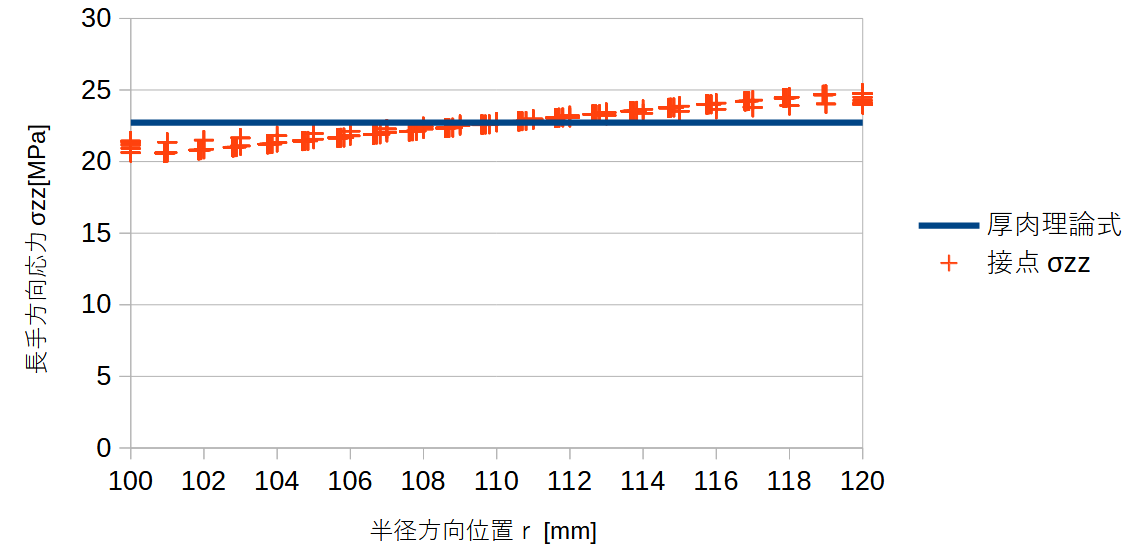
\includegraphics[width=\columnwidth]{work/images/results03.png}
     \caption{長手方向応力
       \begin{math}
         σ_{zz}
       \end{math}
     }
  \end{minipage}
%
  \begin{minipage}{0.49\columnwidth}
  \end{minipage}
\end{figure}
\end{frame}
